% for landscape posters, use "a4paper, landscape"
\documentclass[a4paper]{article}
\usepackage{better_poster}


% ---- fill in from here
% poster size - this will scale the poster to the given size.
% for landscape posters add ", landscape" to the postersize command.
\postersize{a0paper}

% authors
\title{Is the Linear Correlation Between Classification and Rotation/Jigsaw Prediction Model-Invariant?}
\author{Callum Koh}

% type of poster: [exp]erimental results, [methods], [theory]
% Disclaimer: the original classification had "study" and "intervention" as separate categories. I group them under experimental results.
\newcommand\postertype{imperialblue} % [exp],[methods],[theory]

\begin{document}

% main point of your study
\makefinding{
There is a \textbf{Strong Linear Correlation}
\\between \textbf{Image Classification} Accuracy
\\and \textbf{Jigsaw Solving} Accuracy,
\\for \textbf{Almost All} Classification Models
}



% the main text of your poster goes here
\makemain{
    % you can have 1 or 2 columns
    \raggedcolumns
    \begin{multicols}{2}
        \section{Intro}
        \vspace{-0.4cm}
        \begin{compactitem}
            \item Adding labels to images extremely laborious.
            \item Difficult to automate.
        \end{compactitem}
        \begin{compactitem}
            \item Can gauge classification accuracy from rotation/jigsaw accuracy.
            \item \textbf{Linear relationship only shown using one model for one dataset.}
            \item \textbf{Must be tested using fixed dataset and many models.}
        \end{compactitem}
        \vspace{-0.5cm}
        \section{Method}
        \vspace{-0.4cm}
        \begin{compactitem}
            \item[1.] Use CIFAR-10 dataset,
            \item[2.] Take pretrained classification model,
            \item[3.] Fix weights of all layers,
            \item[4.] Train new fully-connected layer for rotation/jigsaw,
            \item[5.] Test classification and rotation/jigsaw on corrupted CIFAR-10 datasets,
            \item[6.] Repeat for 16 other models.
        \end{compactitem}
        
    % this determines where your columns will be separated
    \columnbreak

        \section{Results}
        \vspace{-0.4cm}
        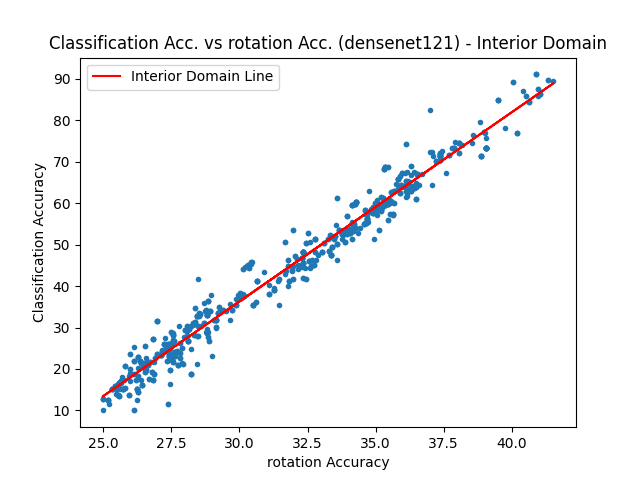
\includegraphics[scale=0.4]{images/sample1.png}
        \begin{compactitem}
            \item Linear correlation observed on both tasks, \textit{for all but one model.}
            \item Even simplest models showed medium to strong fit.
            \item Linear Fit in Interior Domain doesn't always hold in Exterior Domain.
        \end{compactitem}
        \vspace{-0.5cm}
        \section{Future Work}
        \vspace{-0.4cm}
        \begin{compactitem}
            \item Test more models
            \item Apply method to other datasets e.g: ImageNet
            \item Test other self-supervised methods
        \end{compactitem}
    
    \end{multicols}
}
% If you have extra figures or data to show
\makeextracolumn{
    \begin{flushleft}
    Linear Classification - Jigsaw (Simplest)
    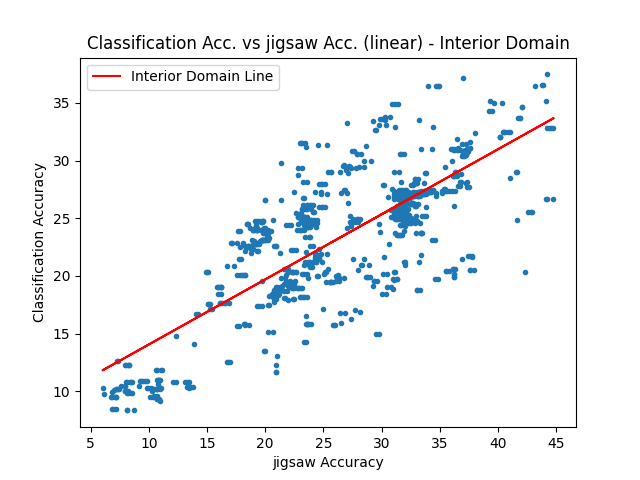
\includegraphics[scale=0.17]{images/sample3.png}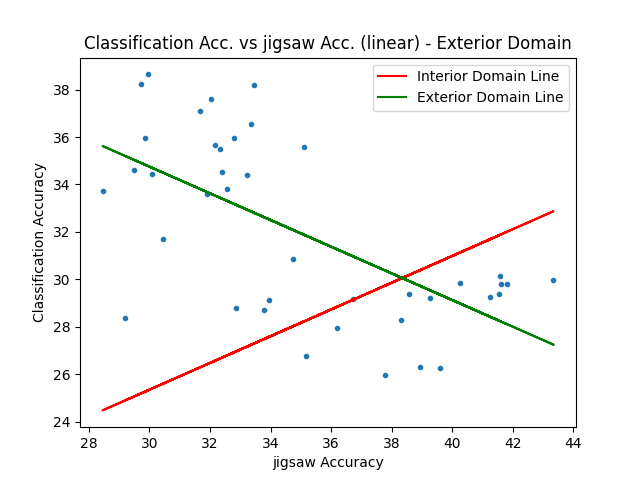
\includegraphics[scale=0.17]{images/sample2.png}
    LeNet5 - Jigsaw
    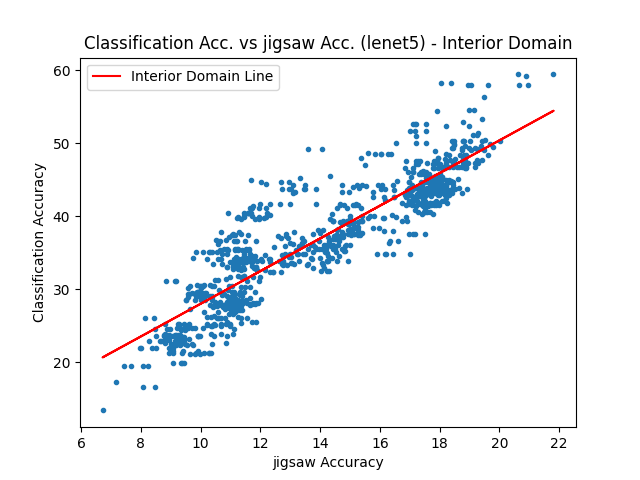
\includegraphics[scale=0.17]{images/sample8.png}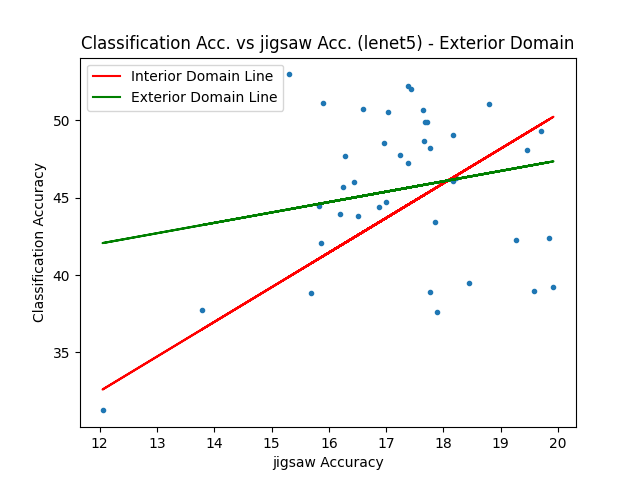
\includegraphics[scale=0.17]{images/sample9.png}
    Inception\_v3 - Rotation
    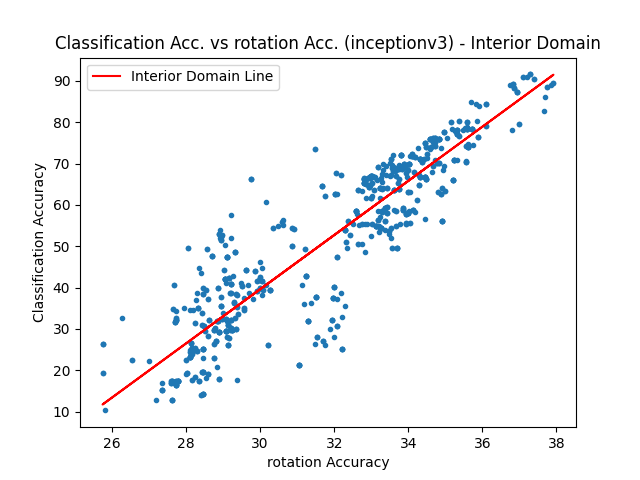
\includegraphics[scale=0.17]{images/sample4.png}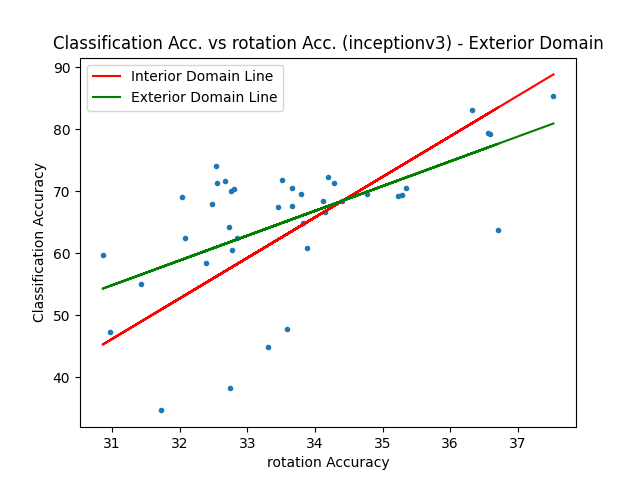
\includegraphics[scale=0.17]{images/sample5.png}
    ResNet1202 - Jigsaw (Most Complex)
    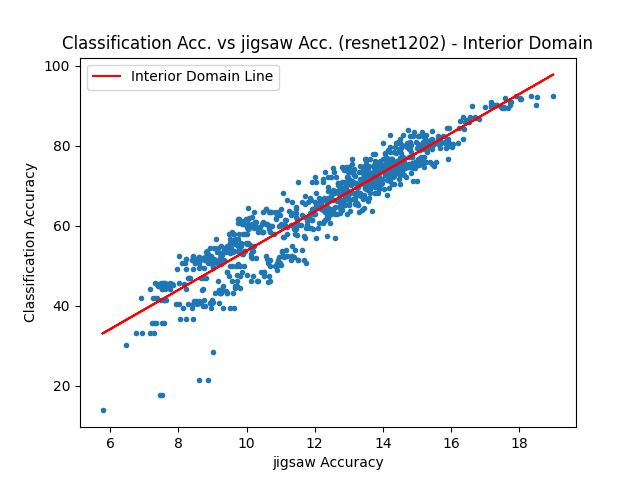
\includegraphics[scale=0.17]{images/sample6.png}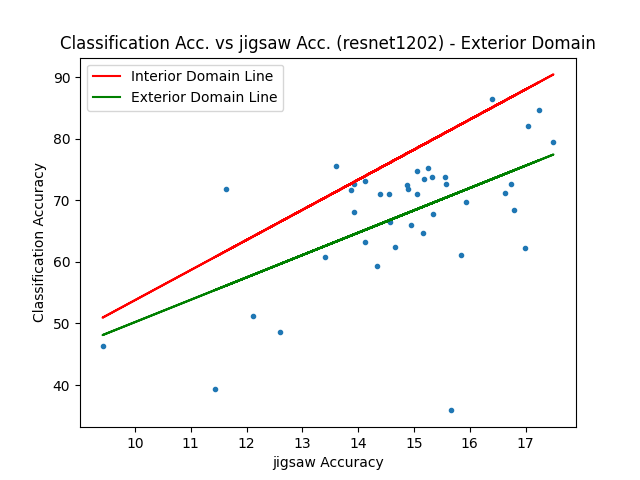
\includegraphics[scale=0.17]{images/sample7.png}

    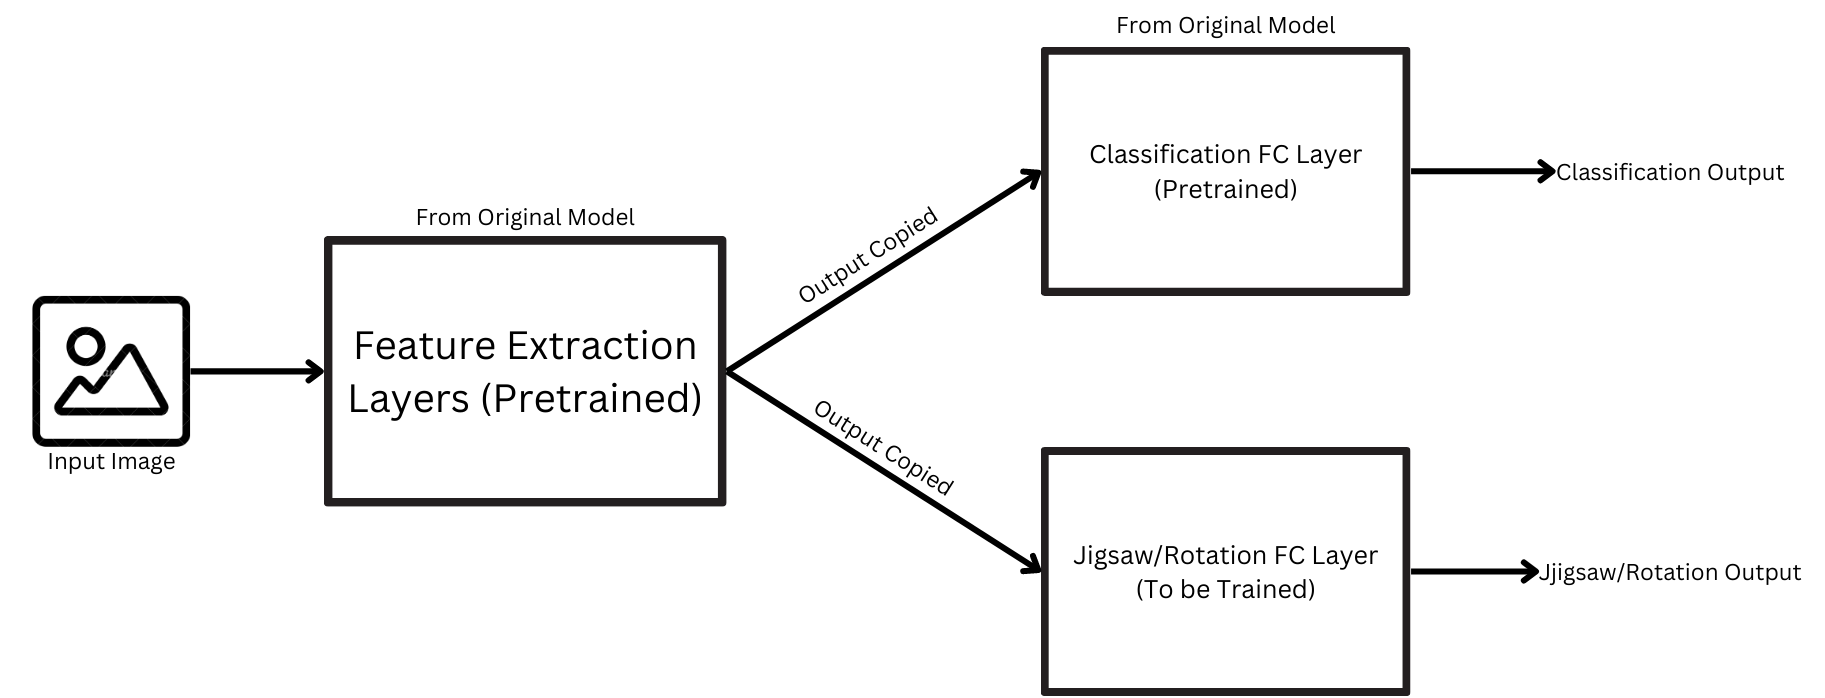
\includegraphics[scale=0.11]{images/diagram.png}

    \vspace{0.3cm}
    Interior Domain = Modified versions of original dataset used for training models in any task.
    
    Exterior Domain = Variants of original dataset eg: CIFAR-10.1.

    \end{flushleft}
}

% footer
% generate qr code from https://www.qr-code-generator.com/ and replace qr_code.png
% default: barcode on the left
\makefooter{images/uni_logo1.png}{images/paperqr.png}
\end{document}